\section{Implementation}
This section concentrates on the usage of the previously mentioned technologies during the development of this web application. In particular, we discuss what parts have been developed in the backend and the frontend, and how each of these have been implemented.

% Backend subsection
\subsection{Backend}
This contained the bulk of the computational work for the re-pairing game. This includes any validations on inputs, calculations on the width property for a re-pairing and the generation of re-pairing moves using strategies.

The majority of functions in the backend were developed to handle \textbf{POST} requests rather than \textbf{GET} requests. This is because the backend is used more so as a way to process any incoming data about Dyck words from the frontend rather than to store data. This decision is a deliberate one, and elaborated on further in the frontend section.

As a result, almost all backend functions with app routes will return data using the \textbf{jsonify} function from the Flask library. This ensures any data is properly formatted in the JSON (JavaScript Object Notation) format. It can take Python data structures, such as lists and dictionaries, and convert them into a string format that can be easily transmitted to and understood by React. It's important to note that not all Python objects can be converted into JSON format. However, for the purposes of this project, all relevant data structures can be converted by jsonify.

We also make use of the \textbf{Flask-CORS} library. CORS stands for Cross-Origin Resource Sharing, and is mechanism used to allow a web application to indicate any domains or ports other than its own from which a browser should permit loading resources\cite{}. The backend runs locally on {`127.0.0.1:8080'}, which is different to the frontend's location at {`localhost:5173'}. This separates the development of the frontend and the backend, allowing each of them to be tested separately before being combined together. However, this means they both run on different origins, and therefore we must use Flask-CORS. 

\subsubsection{Validation}
Given any input, we want to ensure that it is indeed a valid Dyck word. To do so, we simply iterate through a given string, checking that it meets the definition of a Dyck word. In particular, since Python strings can be treated as lists, we pass the input into Python, which then allows us to treat each character as an element of a list. We then treat the list of elements as a sequence, and use the sequential definition of a Dyck word (see \autoref{def:seqDyck}). 

\subsubsection{Generating Steps}
When we want to generate the re-pairing moves using a certain strategy on some given valid input, we use Python. This is done through the following steps:
\begin{enumerate}
    \item Call the selected strategy's relevant function.
    \item To calculate each move, iteratively apply the strategy to the input until an empty string is reached, appending each calculated move into a list.
    \item Send the list of moves to a separate function which calculates the width after applying each move, and the maximum width seen during the play.
    \item Return a final 2D list $[m_{1}, \dots, m_{\frac{n}{2}}]$, where each $m_{i}$ contains: 
    \begin{enumerate}
        \item the $i^{th}$ move $[l_{i}, r_{i}]$ corresponding to the index for the left bracket and right bracket respectively
        \item the width of the word after $m_{i}$
        \item the string for the word after $m_{i}$,
    \end{enumerate}
    in that exact order.
\end{enumerate}

\subsubsection{Strategies}
Each of the Simple, Non-Simple, and Greedy strategies are trivially translated into Python from their algorithmic descriptions seen previously.

\subsubsection{Width Calculation}
As a result of generating steps in the backend, the width calculation is also done here. We iterate over the initially generated list of moves, and calculate the width after applying each move. Given a move $m_{i}$, we have two possible approaches to calculating the width.
\begin{enumerate}
    \item \textbf{Approach 1:} A naive approach, where we apply the move to the current word, and run through the word counting the number of non-empty segments encountered. This can be trivially shown to have $\bigO(n^{2})$ (each move requires running through the word of length $n$, and there are $\frac{n}{2}$ moves).
    \item \textbf{Approach 2:} We can speed this up by analysing adjacent characters around the brackets to be re-paired, rather than calculating a new width value each time. This will require storing the previous width, but since we're iterating over the list of moves in order and calculating the width after each move anyway, this requires no extra effort as we can simply take the previous result each time.
\end{enumerate}
We used approach 2, which requires the following observation.

\begin{observation}
    \label{obs:adjAnalysis}
    Replacing a single bracket with the \texttt{\string_} symbol will either maintain the current width, increase the width by one, or decrease the width by one.
\end{observation}
\begin{proof}
    WLOG consider the sequence of characters ``A\texttt{(}B'' (the same logic applies if the character is a right bracket instead). Then we have 3 cases:
    \begin{enumerate}
        \item A and B are both gaps. Here, replacing a bracket with a gap will mean this sequence of characters will no longer contain a non-empty segment of brackets, so the width will decrease by one.
        \item A and B are both brackets. Here, replacing the bracket with a gap will mean this sequence non-empty segment of brackets will be divided by a gap, breaking this into two segments. Therefore, the width will increase by one.
        \item Exactly one of A and B is a bracket. Suppose A was a bracket (we'll represent this as A), and B was a gap (represented as \texttt{\string_}). Then, the re-pairing will turn this sequence of characters from ``A\texttt{(\string_}'' to ``A\texttt{\string_\string_}''. In this case, there has not been a removal of an existing segment like the first case, nor has there been an introduction of a new gap like in the second case. We can think of the gap on the right as \textit{expanding} out into the middle, shortening the segment of brackets on the left. Therefore the width stays the same. 
        \\ Note that by symmetry, this case is the same as A being a gap and B being a bracket, as our gap now \textit{expands} in the opposite direction.
    \end{enumerate}
    This concludes the proof.
\end{proof}

From here, it suffices to analyse the characters adjacent to the brackets being paired. We visualise a move as turning ``A\texttt{(}B\textsubscript{1}\dots B\textsubscript{2}\texttt{)}C'' into ``A\texttt{\string_}B\textsubscript{1}\dots B\textsubscript{2}\texttt{\string_}C'', where A, B\textsubscript{1} are characters adjacent to ``\texttt{(}'' and B\textsubscript{2}, C are characters adjacent to ``\texttt{)}''. We take the width of the subsequence before the move is made and, by using the adjacency analysis from above, add and subtract to this width as necessary.

However, suppose we were re-pairing the Dyck word ``\texttt{(())}'' using the simple strategy. We immediately notice two edge cases with this analysis that cause some issues:
\begin{enumerate}
    \item The first move would be the indices (0, 3). Using our analysis as above, we'd be considering the subsequence ``A\texttt{(}B\textsubscript{1}\dots B\textsubscript{2}\texttt{)}C''. But since this move takes the outermost brackets, A and C do not exist!
    \item The second move would be the indices (1, 2). However, since this move pairs adjacent brackets, here B\textsubscript{1} and B\textsubscript{2} do not exist either!
\end{enumerate}

For the first case, if a pairing takes an outermost bracket we need only consider its respective inner adjacent character. If this is a gap, the width increases by 1, otherwise the width stays the same.

To implement this in Python, we could use boolean logic to check if our move indices are adjacent or outermost. This tells us which adjacent characters exist, and then we can consider what effects these have on the current width. However, we can circumvent the first issue entirely by the following observation:

\begin{observation}
    Consider the Dyck word $D' = ``\texttt{\string_}D\texttt{\string_}''$ created by \textit{padding} an existing Dyck Word $D$ with gaps on the outside. Then given a re-pairing of $D$ with width $w_{i}$ at move $i$, applying these moves as a partial re-pairing to $D'$ gives width $w'_{i} = w_{i}$ for each move $i$.
\end{observation}

This simplifies the first edge case; instead of having to check if a move takes an outermost bracket, we can simply pad the word from the start with gaps on the outside and apply the same analysis as before. 

For the second case we simply check if a pairing takes adjacent brackets or not. If so, we can consider these to be a single bracket like our analysis in the proof of \autoref{obs:adjAnalysis}, and the same idea applies.

Using approach 2 over the naive idea from approach 1 means we do not have to iterate over the string of length $n$ for each of the $n/2$ moves, and instead we require a constant number of steps. This means approach 2 has $\bigO(n)$, which is a quadratic speedup over approach 1.

% Frontend subsection
\subsection{Frontend}
This section explores the higher-level design aspects of the yehweb application. We'll discuss the different components that make up the web application in both the UI and the backend.

It's important to note that most of the data and calculations from the backend on Dyck words are stored in state variables. This allows for a simpler development process; by checking for changes in state variables, re-renders can be made more streamlined since React will re-render automatically when a change to its state variables is made. 

\begin{figure}[H]
    \centering
    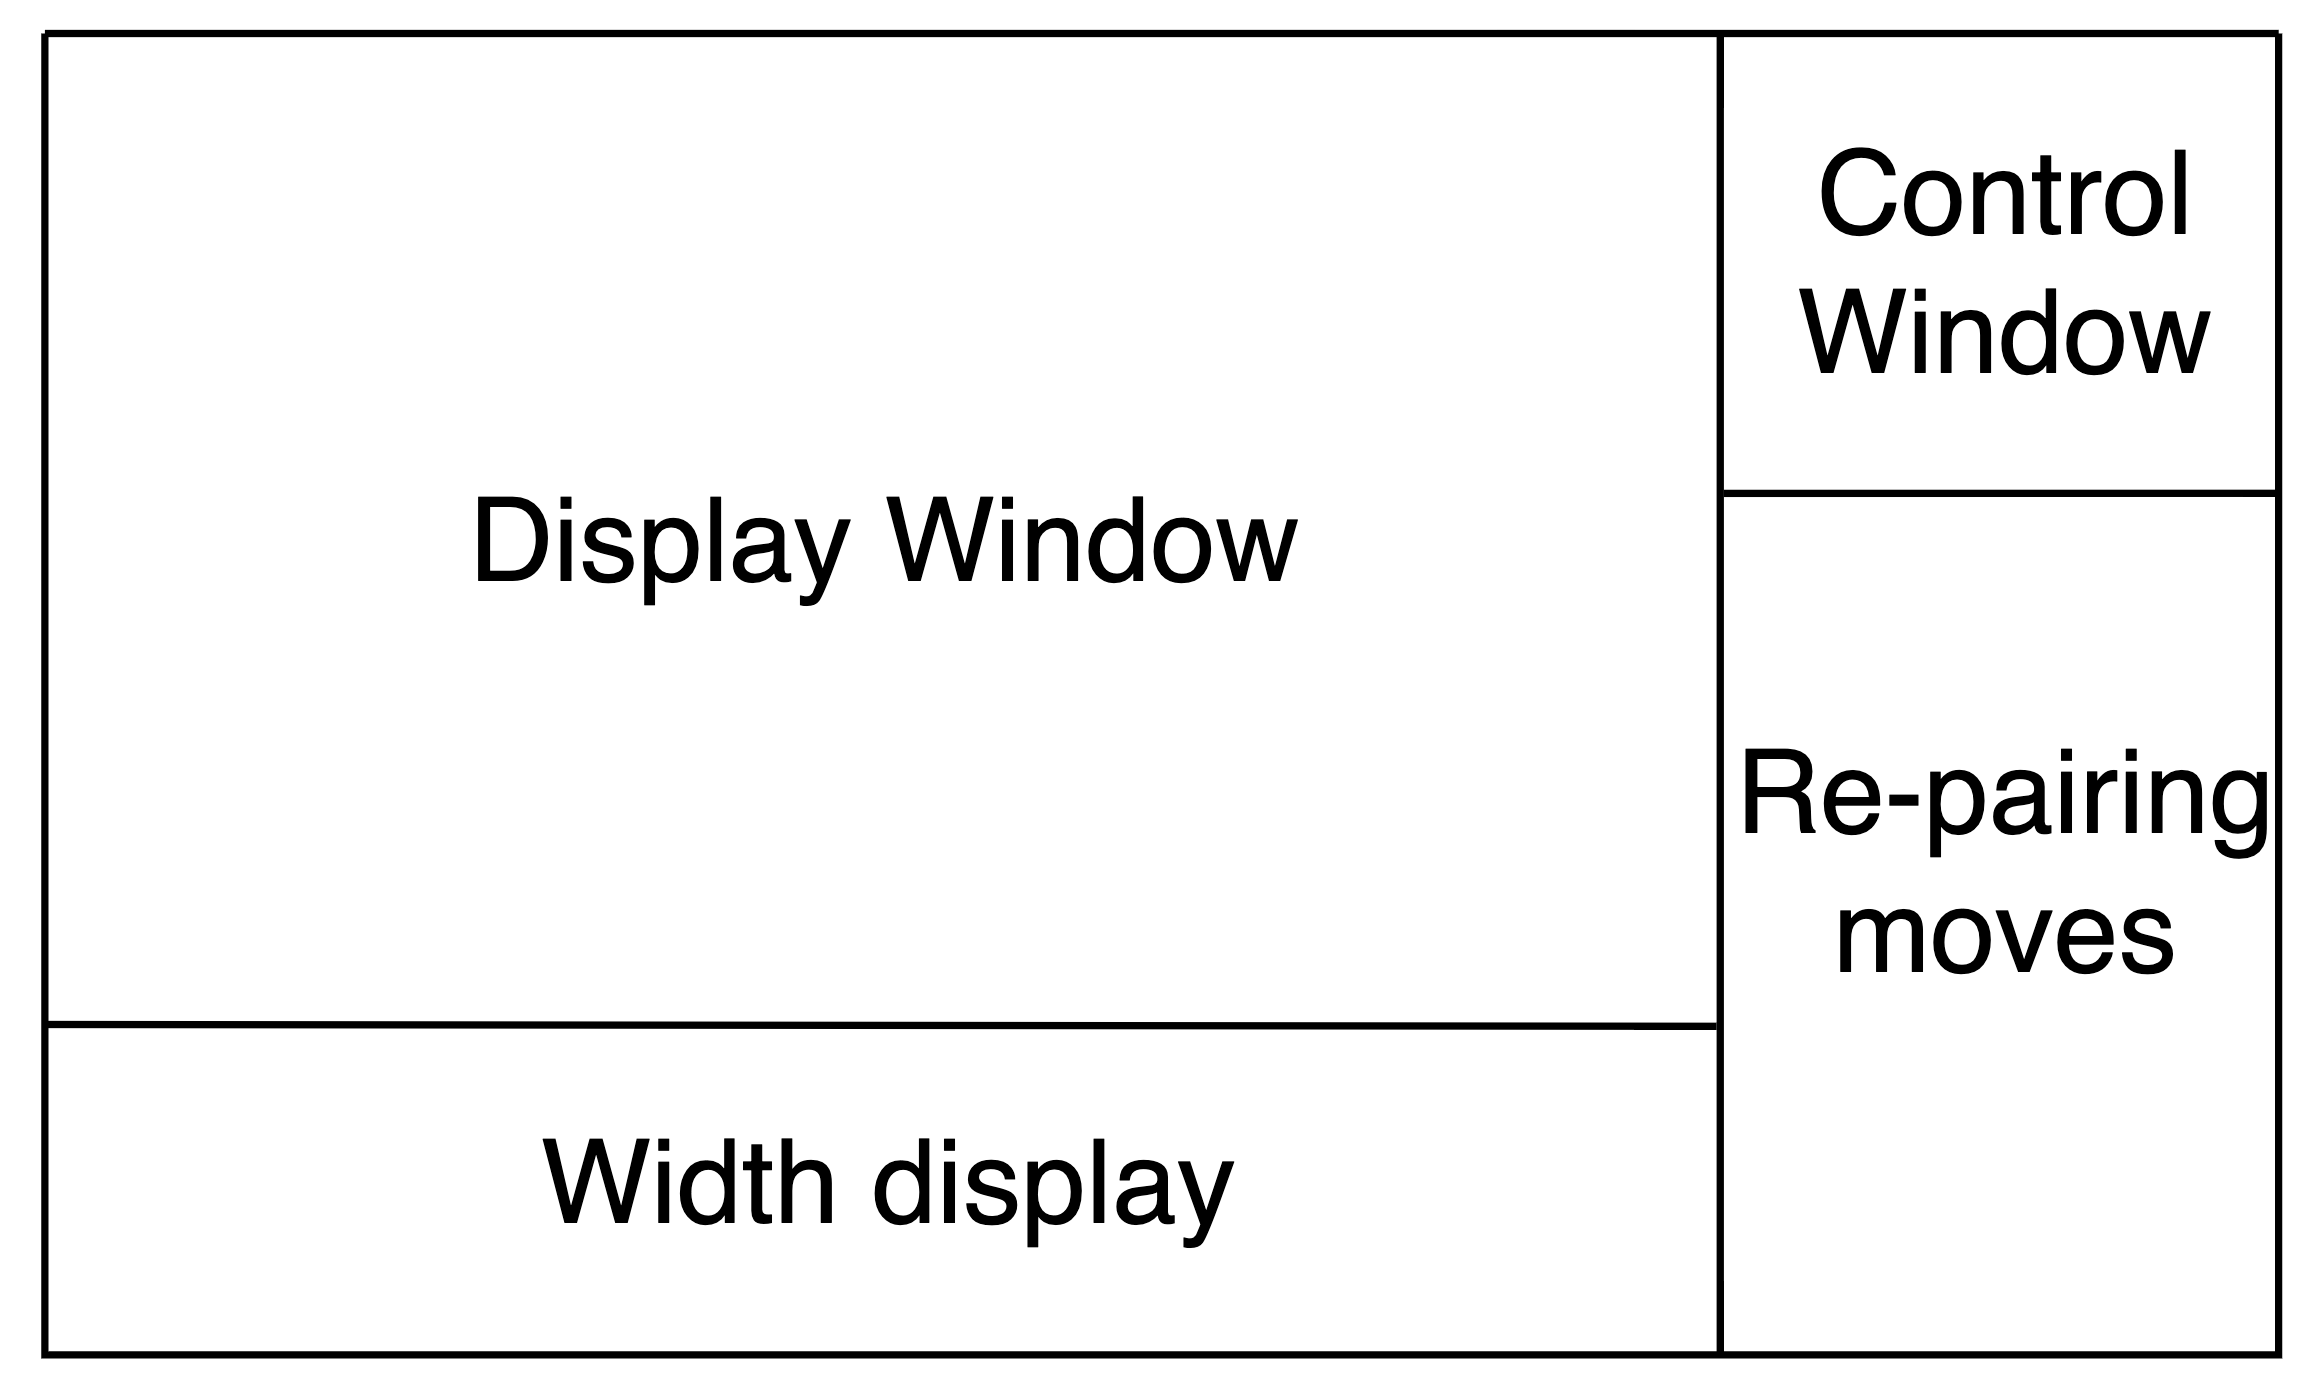
\includegraphics[scale=0.1]{./figures/webBreakdown.png}
    \caption{A high-level overview of the components that make up the web application}
\end{figure}

\subsubsection{Control Window}
This is where all input and controls will exist. Here the Dyck word will be taken in as input, and all options for runnings strategies
